% -*- coding: utf-8 -*-
%%
%%  本模板可以使用以下两种方式编译:
%%     1. PDFLaTeX
%%     2. XeLaTeX [推荐]
%%  注意:
%%    1. 在改变编译方式前应先删除 *.toc 和 *.aux 文件,
%%       因为不同编译方式产生的辅助文件格式可能并不相同。

%\documentclass{cumcmart}
\documentclass[nocover]{cumcmart}%%
%切换到无封面的版本,有些赛区不允许前面的承诺页用pdf格式,可以用此选项去掉。

%\usepackage[refsection=section]{biblatex}
\usepackage{listings}
\usepackage{cite}
\begin{document}


\title{关于多人同心鼓游戏中最优协作策略的研究}

\xuanti{A}
%\school命令用于在承诺书上显示学校名称。按要求,此处应填写全称
\school{XXXX大学}
%以下命令分别显示队员及指导教师姓名
\numbers{2010888}%参赛报名号
\authorone{队员1}
\authortwo{队员2}
\authorthree{队员3}
\advisor{数模指导组}

\newcommand{\lhp}[1]{\textcolor{cyan}{lhp: #1}}
\newcommand{\znq}[1]{\textcolor{blue}{znq: #1}}

%\theyear{2010}

\theday{16}%填写当月的具体日期

\maketitle
\begin{cnabstract}%此处没有采用sbstract命名,是为了将来如果要加入英文摘要时扩展的方便

同心鼓游戏是一个以团队挑战为主的项目,对团队成员的团结协作能力有很大要求,在实际的素质拓展活动中常常被采用。本文基于颠球次数尽可能多的目标,对该项目中球与鼓的受力与运动进行研究,综合考虑人的反应能力、控制能力等综合生理要素,建立符合该项目进行过程的物理模型,研究团队成员的最佳行动方案。

对于问题1,该问题针对理想状态下,每位团队成员都可以精确控制用力方向、时机和力度的情况。此状态下球与鼓都只进行匀加速直线运动,且鼓面可以始终保持水平。我们定义最佳方案为能量消耗最小的方案,即使得每次颠球高度为最小合法高度。在此基础上,我们建立球与鼓的运动模型,利用牛顿第二运动定律与动量守恒定律,运用MATLAB计算出不同恢复系数下团队成员拉绳的力度与周期。

对于问题2,该问题针对现实情形中,队员发力时机和力度不可能做到精确控制,存在一定误差,于是鼓面可能出现倾斜。我们建立鼓与球的运动模型,首先计算鼓的转动惯量,然后使用角动量定理计算出鼓的角加速度。在此基础上,我们列出动力学方程,运用MATLAB计算鼓面的转动角度。我们发现所有情况下,旋转角的值都比较小。这印证了我们模型设计的合理性。同时,对于旋转角产生因素的研究也为我们在问题3中进行优化创设了条件。

对于问题3,由于问题2中误差存在,我们需要将其进行修正,尽量使鼓面保持水平。我们在人类正常反应时间、控制能力的基础上,认定团队成员可以分辨鼓朝向其方向旋转或朝向其反向旋转,可以分辨鼓旋转的速度为快或慢,要求各团队成员加大力度或减少力度。我们将我们的优化后的模型运用在问题2的数据集上,使用MATLAB分别计算优化后、优化前全过程的鼓面旋转角。实验结果表明,优化后的模型保证最终状态的角速度较小,继而当球不精准落在鼓心时,可以减少对于球的运动所造成的影响。

对于问题4,我们需要在给定条件下对鼓面进行调整。我们对鼓的运动进行分析,在人类正常反应时间、控制能力、视觉能力的基础上,要求团队成员采取不同的力度,让鼓进行角加速度运动,进而对鼓面的倾斜角误差进行修正。


\cnkeywords{同心鼓游戏,优化模型,协作策略,微分法}
\end{cnabstract}

\newpage
%\tableofcontents\newpage%增加目录,要不要都可以。不想要的话,就在本行前加“%”(英文的百分号)


\section{问题重述}
\subsection{问题背景}
“同心协力”(又称“同心鼓”)项目考察团队协作能力。该项目要求团队成员使用一牛皮双面鼓,鼓身一圈固定多根长度相同的绳子,绳子的固定点沿圆周均匀分布。每条绳子的另一头由一位团队成员牵拉,控制整条绳,并通过绳子共同控制鼓。

项目开始时,球从鼓面中心上方竖直落下,队员共同控制绳子,让鼓将球颠起,使其有节奏地在鼓面上跳动。颠球过程中,队员只能抓握绳子的末端,不能接触鼓或绳子的其他位置。

项目所用排球的质量为 270 g。鼓面直径为 40 cm,鼓身高度为 22 cm,鼓的
质量为 3.6 kg。队员人数不少于 8 人,队员之间的最小距离不得小于 60 cm。项目开始时,球从鼓面中心上方 40 cm处竖直落下,球被颠起的高度应离开鼓面 40 cm 以上,如果低于 40 cm,则项目停止。试探索策略,使得项目结束时,总共颠球次数尽可能的多。

\subsection{提出问题}
问题1:在理想状态下,每位团队成员都可以精确控制用力方向、时机和力度,试讨论
这种情形下团队的最佳协作策略,并给出该策略下的颠球高度。

问题2:在现实情形中,队员发力时机和力度不可能做到精确控制,存在一定误
差,于是鼓面可能出现倾斜。试建立模型描述队员的发力时机和力度与某一特定
时刻的鼓面倾斜角度的关系。设队员人数为 8,绳长为 1.7m,鼓面初始时刻是水
平静止的,初始位置较绳子水平时下降 11 cm,表 1 中给出了队员们的不同发力
时机和力度,求 0.1 s 时鼓面的倾斜角度。

问题3:在现实情形中,根据问题 2 的模型,对问题1中的模型进行合适的调整。

问题4:当鼓面发生倾斜时,球跳动方向不再竖直,于是需要队员调整拉绳策略。
假设人数为 10,绳长为 2m,球的反弹高度为 60cm,相对于竖直方向产生 1 度
的倾斜角度,且倾斜方向在水平面的投影指向某两位队员之间,与这两位队员的
夹角之比为 1:2。为了将球调整为竖直状态弹跳,请给出在可精确控制条件下所
有队员的发力时机及力度,并分析在现实情形中这种调整策略的实施效果。

\section{问题分析}
在同心鼓游戏中,为了使颠球的次数尽可能的多,多位团队成员需要齐心协力,尽可能使鼓表面保持水平。因此,团队成员应当尽量将每次颠球的发力时机控制在同一时刻。并且,在球距离鼓面高度需大于40cm的条件下,团队成员应当尽量将球的颠起高度控制在40cm,不需要过高,以节省力气,保证更多的颠球次数。

对于问题1,我们考虑每个人都可以精准控制用力方向、时机和力度的理想状况。为了使颠球次数尽可能多,我们要求团队成员每次将球颠起的高度恰好为40cm,即合法的最小高度。这是一个最节省能量的方案,我们也将此认定为最优方案。

对于问题2,考虑到实际情况下,某些人发力的时间和力度可能会有一定误差,我们计算误差情况时,对鼓的表面所造成的倾斜影响。在此问题中,首先计算鼓的转动惯量,然后使用角动量定理计算出鼓的角加速度。在此基础上,我们列出动力学方程,计算鼓面的转动角度。

对于问题3,由于问题2中认定团队成员的操作可能存在力度、时间上的误差,我们根据人类正常的反应时间与控制能力,认为团队成员可以分辨鼓朝向其方向旋转或朝向其反向旋转,可以分辨鼓旋转的速度为快或慢,可以选择加大力度或减少力度,分别对应着加大或减少50\%的力。我们将拉绳的过程分为三个部分,分别为失误拉绳、正常拉绳与失误修正三个阶段,对每个阶段沿用问题2中的模型。

对于问题4,我们需要在在给定条件下,对鼓面进行调整。我们将鼓的运动分为三个过程,自由落体、匀加速与调整角度。前两个过程我们沿用问题1的模型,调整角度过程我们认为鼓作匀角加速旋转,列出受力方程并进行求解。

\section{模型假设}

\begin{enumerate}
    \item 不考虑球的形状与体积,将球视为质点。
    \item 不考虑绳的弹性与质量,将绳视为轻绳。
    \item 不考虑鼓上表面的曲率,将鼓上表面视为二维平面。
    \item 不考虑球和鼓运动过程中的空气阻力。
    \item 将鼓视为薄壁圆桶。
    \item 假设每个人牵拉绳时手的位置在同一平面上。
    \item 假设每条绳子的固定点到牵拉者手的距离相同。
    \item 假设任意相邻两条绳子所成的夹角相同。
\end{enumerate}

\section{符号}
我们在表\ref{table:symbol}此列出本文中会用到的所有符号,并声明其含义。
\begin{table} [!h]
\begin{center}
\vspace{-0.1in}
\caption{本文中用到的符号}
\label{table:symbol}
\begin{tabular}{|c|l|}
\hline
\textbf{符号}&\textbf{含义}\\
\hline
$e$&球和鼓面碰撞后的恢复系数\\
\hline
$I$&鼓面的转动惯量\\
\hline
$v_0$&球与鼓面碰撞后的初速度\\
\hline
$M$&鼓的质量\\
\hline
$m$&球的质量\\
\hline
$\beta$&受到外力时鼓面的角加速度\\
\hline
$\delta$&外力对鼓面造成的旋转角度\\
\hline
$\omega$&鼓面转动的角速度\\
\hline
$T$ &整个过程的周期\\
\hline
$\theta_i$ &第$i$条绳与y轴的夹角\\
\hline
bias &角偏量,定义为$\theta_i - \frac{\pi*i}{4}$\\
\hline
$J_i$ &第$i$条绳子作用给鼓的力矩\\
\hline
$J$ &所有绳子作用给鼓的合力矩\\
\hline
\end{tabular}
\vspace{-0.2in}
\end{center}
\end{table}


\section{模型建立与求解}
\subsection{问题1:最理想状态}
\subsubsection{建立模型}
在理想状态下,我们假设每个人的发力时间和力度都可以被精准控制。因此,我们首先要求所有人的发力时间一直,力度大小相同。在此基础上,
考虑最优解,我们认为题意对于球上升高度的要求是指球与鼓之间的相对高度差不低于0.4m,因此选取使得球弹起最小的高度,即球与鼓之间的相对距离的最大值为0.4m,显然这是一个最节省能量的方案。除此之外,由于球上升的距离最小,这个运动的周期也是最小的,这也可以在单位时间内进行弹起最多的次数。

我们在这里建立如下的模型:

所有人围成一圈,使得每个人抓住绳子的手的位置均匀分布在一个正多边形的各个顶点。绳子另一端均匀分布在鼓的四周,将之抽象为图\ref{5.1.1 模型抽象示意图}所示。
\begin{figure}[h!]
    \centering
    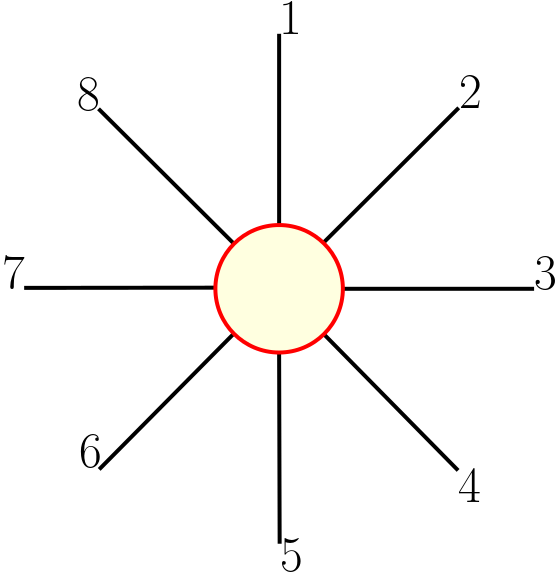
\includegraphics[width=0.4\linewidth]{figures/f1.png}
    \caption{5.1.1 模型抽象示意图 (8人情况)}
    \label{5.1.1 模型抽象示意图}
\end{figure}

我们首先分析球的一系列运动。球每次与鼓碰撞之后,首先进行竖直上抛运动,当速度减为0时,再进行自由落体运动。当球落下至初始位置时,会与鼓再次相碰,重复刚才的一系列运动。
球的运动是周期运动。

我们接下来分析鼓的一系列运动。鼓每次与球碰撞之后,首先进行竖直上抛运动,当速度减为0时,再进行一段自由落体运动。该过程绳子保持松弛。当绳子绷紧时,自由落体运动结束,
随后由于团队成员所施加外力的影响,鼓在某一位置$y_{d1f}$开始进行加速度恒定、方向竖直向下的匀减速直线运动,直至速度减为0。接下来,由于团队成员所施加外力的影响,鼓以相同的加速度进行向上的匀加速直线运动,到达碰撞的位置,与球进行碰撞。
鼓的运动也是周期运动。

在此模型中,我们假设所有团队成员在相同的时刻,位于相同的高度拉绳子,并在鼓与绳子碰撞的瞬间松开绳子使其自由落体。此外,所有团队成员均能够准确的控制拉绳子的力与时间,并且同一时刻每个团队成员施加的力大小相等,与竖直方向所成的夹角相等。在求得鼓与球的运动学规律之后,我们可以基于此假设求得每个团队成员在整个过程中任意位置的力的大小与方向。
\subsubsection{模型求解}
现在我们对该模型进行求解\cite{力学}。

\begin{enumerate}[(a)]
\item
球与鼓运动周期的时间记位$T$,则
$$T = \frac{2v_0}{g}$$
    \item
    鼓竖直上抛的过程经过t1结束,则
    $$y_{d1f} = v_{1i}t1 - \frac{1}{2}g t_1^2$$
    $$v_{1f} = v_{2i} = v_{1i}-gt1$$
    \item
    鼓进入匀加速直线运动状态,经过t2回到初始状态,则
    $$0 = y_{d1f} + v_{2i}t2 + \frac{1}{2}a t_2^2$$
    鼓与球之间的最大距离为$\Delta H = 0.4$m
    $$\Delta H = (v_0 - v_{1i})t1 + \frac{(v_0 -v_{1i})^2}{2(g+a)}$$
    $$v_{2f} = v_{2i} + a_2 t_2$$
    $$T = t1 + t2$$
    \item
    考虑碰撞的过程,设恢复系数为e,则考虑动量守恒与恢复系数的定义可以得到
    $$m v_0 + M v_{1i} = M v_{2f} - m v_{0}$$
    $$v_0 - v_{1i} = e(v_0 + v_{2f})$$
    \item
    不妨设绳长为L,球与鼓发生碰撞的位置距离团队成员手所在的平面$h_0$,不妨以竖直向上为正方向,当鼓位于$y_d$时,由于拉力必然沿绳方向,故拉力与水平面的夹角为(以向上的角为正),
    $$\theta = \arcsin{\frac{y_d - h_0}{L}}$$
    拉力满足动力学方程
    $$n T \frac{-y_d}{L}-Mg = Ma$$
    解得
    $$T = \frac{-ML(a+g)}{n (y_d - h_0)}$$
   
    此处当鼓与球相碰之后,T将小于0,但是此时鼓处于竖直上抛的状态,因而此矛盾不存在。
    
\end{enumerate}

整个过程的运动可参照图\ref{5.1.1 球与鼓运动示意图}。

\begin{figure}[h!]
    \centering
    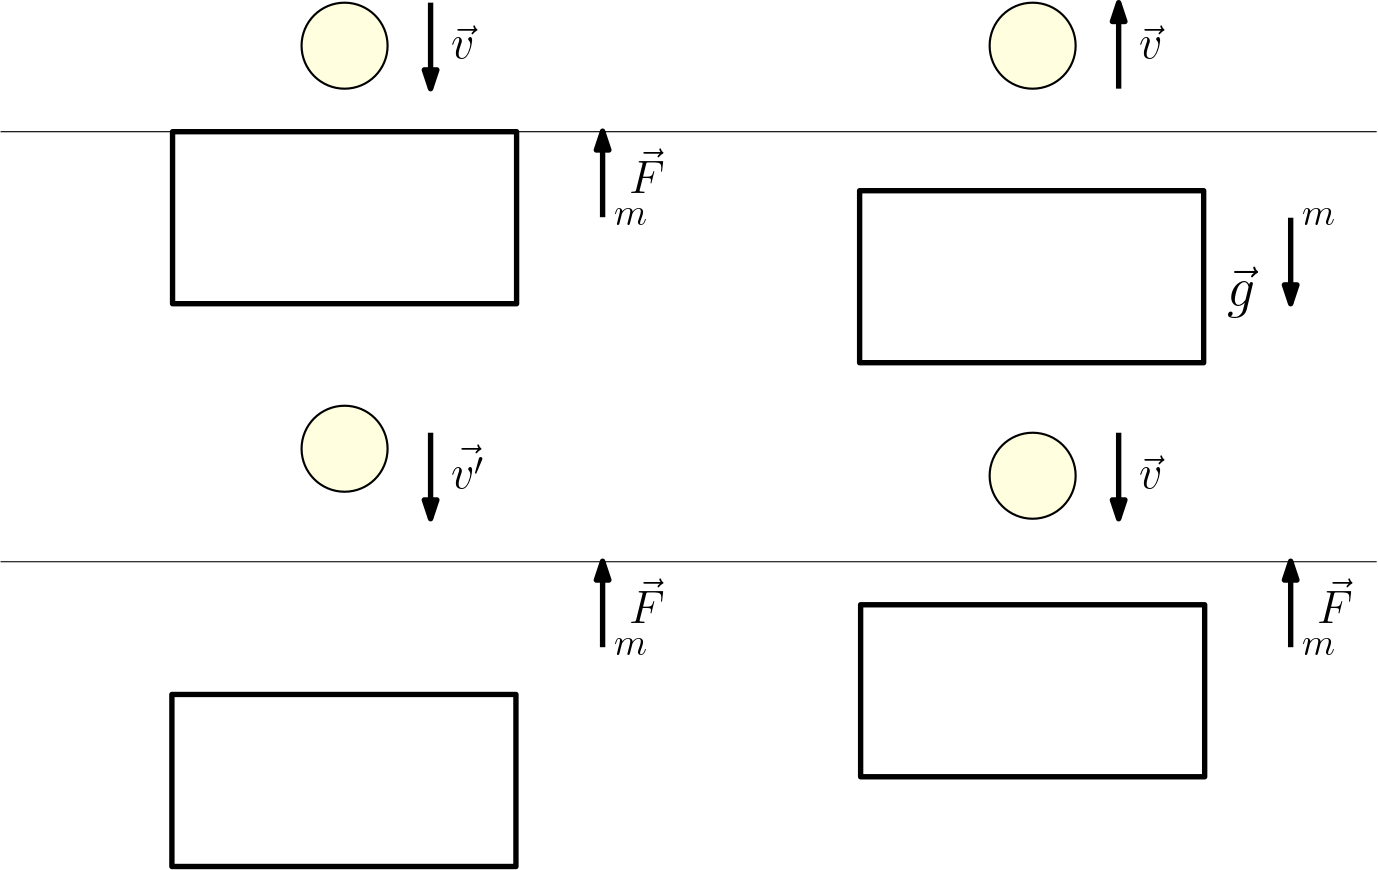
\includegraphics[width=0.65\linewidth]{figures/3.png}
    \caption{5.1.1 球与鼓运动示意图}
    \label{5.1.1 球与鼓运动示意图}
\end{figure}

我们根据一定的化简之后,使用MATLAB求其数值解,求解代码如附录中问题1代码所示。\cite{matlab应用}
我们不妨对于$e = 0.7, n = 8$为例进行求解,
可得$T_0=0.5162$,球的上抛高度为0.653m。

\subsection{问题2:非理想状态,计算短时间内鼓面倾斜角度}
\subsubsection{建立模型}
由于鼓受到团队成员拉绳的作用时间与力的大小存在差别,其在质心运动的同时,也会收到一个相对于质心的净力矩,因此鼓面会产生一定大小的角速度,与初始状态所在平面产生一定夹角。在产生夹角的同时,每根绳的受力方向也可能发生变化。我们考虑外力对鼓的质心所产生的力矩,计算出来鼓旋转的角加速度,进而使用时间微元法,认为在每一微元时间内,角度,角速度,角加速度均为定值。

该过程分析如下\cite{力学zkh}:

\begin{enumerate}[(a)]
    \item 
计算转动惯量$I$:

我们将鼓视为匀质薄壁圆筒,同时忽略上下表面(鼓皮)的质量。同时根据题目图片所示,我们假定绳子连接在鼓侧壁母线的中点处,我们假设鼓的旋转就是沿着母线中点所在水平轴的旋转,这一轴同时通过质心,由此建立坐标系,求鼓相对于此轴的转动惯量$I$,具体代码如附录中问题1代码所示。

%\znq{来一个超链接至附录的I.m的位置}

$$I = \iint {\rm d}m(y^2 + z^2) = \iint  r{\rm d}\theta {\rm d}z (z^2 + r^2 \sin{\theta}^2) = 0.0865 kg\cdot m^2$$
\item 估算只有一个力,经过0.1s可以对于鼓产生的影响,
\begin{enumerate}[(1)]
    \item 假设旋转角度较小,可以忽略力水平分量对于旋转轴的力矩,只考虑力竖直分量产生的影响,此时
    $$\vec{J} = \vec{r}\times \vec{F}$$
    $$|\vec{J}| = rF\alpha = 1.035 N\cdot m$$
    \item 根据角动量定理,此时的角加速度为
    $$\beta = \frac{M}{I} = 11.97 s^{-2}$$
    \item 假设其匀角加速度运动,在0.1s内可以转过的角度为
    $$\delta = \frac{1}{2}\beta \Delta t^2 = 0.06 rad$$
    \item 由此可见,这个角度与其所受拉力与水平面的夹角相比,仍然是一个很小的量,这意味着我们之前忽略力水平分量的假设是合理的。
\end{enumerate}
\end{enumerate}

由此我们可以看出,在加速的第一阶段,旋转角达到最大时,也只有0.06 rad,该角度依然很小。由于鼓的半径与绳子的长度相比很小,我们便可以忽略在这个过程中,力的方向的变化。我们计算的过程允许了非小角的存在,因此即使算出较大的旋转角,也是合理的结果。

因此,我们建立如下的模型:

我们将产生误差的情况分为两种:对称的情况与非对称的情况。对称的情况定义如下:拉绳时间不同与拉绳力度不同在同一方向发生。在这种情况下,两种误差所带来的影响是同方向的,我们可以认为鼓围绕某一轴做定轴转动;非对称的情况定义如下:拉绳时间不同与拉绳力度不同在不同方向发生。在这种情况下,两种误差所带来的影响是不同方向的,我们应该研究刚体的定点转动。

事实上,我们在完成对于对称情况的模型求解后,发现不论是提早0.1s开始发力,还是力的大小较其他队员较大,在0.1s内所转过的夹角都是一个相当小的结果,我们可以将其视为角度微元\cite{力学},角度微元可以被看作矢量\cite{力学},满足平行四边形叠加原理。我们在处理非对称情况时,将其分成两个对称的情况进行处理,随后进行矢量叠加。

\subsubsection{模型求解}
我们首先求解对称的情况,这种情况下鼓进行定轴转动。
不妨根据定轴转动的轴对于不同的受力点进行编号。此处我们将定轴转动的轴规定为拉力对称轴通过圆心的垂线。在此基础上,我们建立三维坐标系:$y$轴为旋转轴,正方向朝向纸面外;$z$轴垂直于鼓面初始状态所在平面,正方向为竖直向上;$x$轴由$y$轴、$z$轴共同确定,三条轴的分布满足右手定则。参照图\ref{5.2.1 三维坐标示意图}。

\begin{figure}[h!]
    \centering
    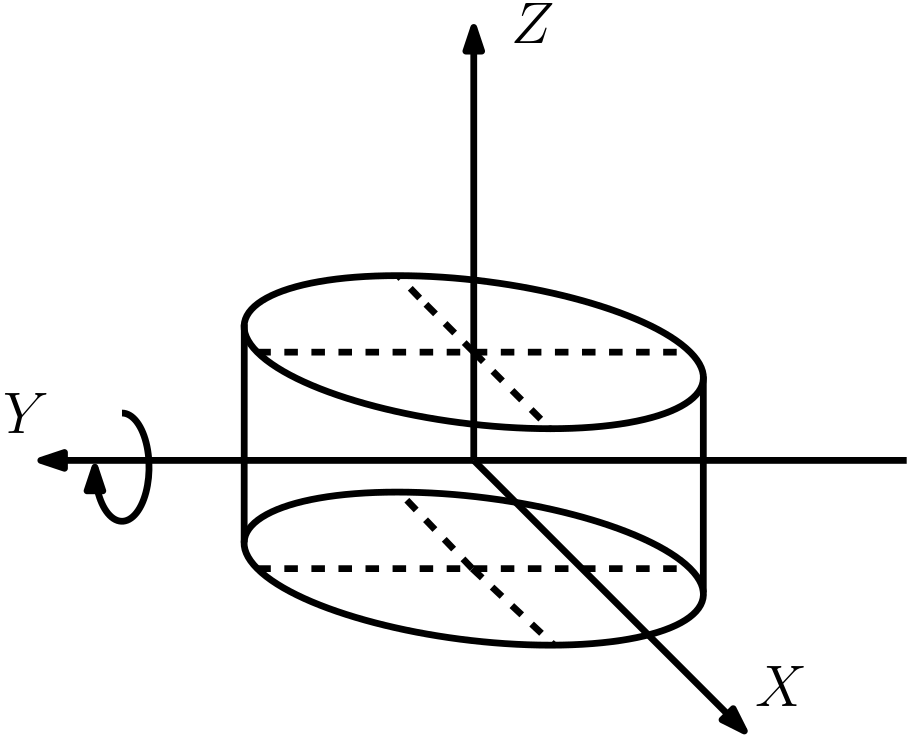
\includegraphics[width=0.4\linewidth]{figures/f2.png}
    \caption{5.2.1 三维坐标示意图}
    \label{5.2.1 三维坐标示意图}
\end{figure}
\begin{enumerate}[(a)]
    \item 

利用在问题1中已经求得的转动惯量,我们列出如下的动力学方程
$$|\sum_{i = 1}^{n} \vec{J_i}| = I\frac{d\omega}{dt}$$

\item
不妨设鼓面转过角度为$\delta$。在建立模型时,我们已经证明了角度转动很小,但是为了得到更加准确的结果,我们仍然考虑不同位置的不同$\delta$的情况。
$$\omega = \frac{{\rm d}\delta}{{\rm d}t}$$

\item
此处的代码我们用到了一个变量bias。这里的bias定义为
$$bias = \theta_i - \frac{\pi*i}{4}$$
即每条绳子与其所对应的原始位置的角度之差。

\item
现在我们计算每一条绳子受力点的坐标与三个方向上的受力情况。

$$\vec{r_i} = (r\sin{\theta_i}\cos{\delta}, r\cos{\theta_i}\cos{\delta}, r\sin{\delta})$$
$$\vec{F_i} = (F\sin{\theta_i}\cos{\alpha}, F\cos{\theta_i}\cos{\alpha}, F\sin{\alpha})$$
$$\vec{J_i} = \vec{r_i} \times \vec{F_i}$$
\item
这里我们使用微元法,将时间分割成小时间段的方法进行数值模拟,即
$$\omega(t+\Delta t) = \omega(t) + \frac{|\sum_{i = 1}^{n} \vec{J_i}|}{I} \Delta t$$
$$\delta(t+\Delta t) = \delta(t) + \omega \Delta t$$

\end{enumerate}
只需要求出每个位置的总力矩,就可以对其进行数值模拟,代码如附录中问题2代码所示。

%\znq{这里跑一下Problem2.m,输入的F, activate, bias等数据位于Prob2data.txt文件中}
计算结果如表\ref{table:result}所示。其中,序号顺序与题目一致。我们规定,如图所示,以旋转轴朝向纸面外的方向为$y$轴正方向,以满足右手定则朝向$y$轴正方向的旋转方向为旋转的正方向。计算结果中,正值为旋转正方向的同方向,负值为旋转正方向的反方向。
\begin{table} [!h]
\begin{center}
\vspace{-0.1in}
\caption{问题2对称情况计算结果}
\label{table:result}
\begin{tabular}{|c|c|}
\hline
\textbf{序号}&\textbf{鼓面倾角 (rad)}\\
\hline
1&-0.0029
\\
\hline
2& -0.0053\\
\hline
3& -0.0020
\\
\hline
4&-0.0154\\
\hline
5&-0.0186\\
\hline
6&-0.0166\\
\hline
7&-0.0103
\\
\hline
9&0.0126
\\
\hline
\end{tabular}
\vspace{-0.2in}
\end{center}
\end{table}     

对于序号8的非对称情况,将其拆分成
\begin{enumerate}[(a)]
    \item 1号和4号队员用力大小较大,bias = $-\frac{\pi}{8}$
    
    采用同上的方法进行计算,转过的角度delta1 = -0.0029rad。
    \item 2号和5号队员发力时机较早,bias = $-\frac{3\pi}{8}$
    
    采用同上的方法进行计算,转过的角度delta2 = 0.0272rad。
\end{enumerate}
接下来将其利用平行四边形法则合成,总共转过的角度为,
$$delta_8 = \sqrt{|delta1|^2 + |delta_2|^2 - 2\cos{(\frac{\pi}{4})}|delta_1||delta_2|}$$
解得,
$$delta_8 = 0.0293rad$$
因此,本题的完整答案如表\ref{table:result2}所示。

\begin{table} [!h]
\begin{center}
\vspace{-0.1in}
\caption{问题2最终计算结果}
\label{table:result2}
\begin{tabular}{|c|c|}
\hline
\textbf{序号}&\textbf{鼓面倾角 (rad)}\\
\hline
1&-0.0029
\\
\hline
2& -0.0053\\
\hline
3& -0.0020
\\
\hline
4&-0.0154\\
\hline
5&-0.0186\\
\hline
6&-0.0166\\
\hline
7&-0.0103\\
\hline
8&0.0293\\
\hline
9&0.0126\\
\hline
\end{tabular}
\vspace{-0.2in}
\end{center}
\end{table}     

\subsubsection{模型分析}
我们发现所有情况下,旋转角的值都比较小。这印证了我们模型设计的合理性。但同样,我们也可以看到,旋转角的结果严重依赖于团队成员的操作,不同的失误会带来各种各样的误差。这也对我们在问题4中进行模型优化创设了提升空间。
\subsection{问题3:现实情形,考虑较长时间内鼓面的倾斜}
\subsubsection{建立模型}

鼓进入匀减速直线运动的过程时的速度为$v_{2i} = -0.60 ms^{-1}$,位置为$y_{d1f} = -0.01m$,加速度为$a = 3.0ms^{-2}$,因此再经过$\delta t = -\frac{v_{2i}}{a} = 0.2s$后,鼓到达最低位置,此位置为

$$y_{dlow} = y_{d1f} + v_{2i}\delta t + \frac{1}{2}at^2 = -0.06m$$

这意味着整个过程中鼓最多相对碰撞位置下降6cm,这与问题2中的11cm同量级,我们可以借助问题2的方法,认为在此问题中鼓处于14cm处,便可以得到一个同量级的估算结果。

我们发现,如果不加任何修正,对于问题2中的情形,如果沿用问题1中建立的模型,由于0.1s后残余的可观的角速度,经过长达0.5s量级的旋转,会在下一次碰撞前达到巨大的旋转角度,继而将球碰偏。为了解决这个问题,我们努力减少碰撞前转过的角度,并尽量减少碰撞时其旋转的角速度,尽最大可能减少其对于碰撞的影响,同时消减其对于下一周期所产生的消极影响。

问题3与问题2不同的是,当考虑系统长时间的过程时,可观的角速度可能使其旋转角度不可忽略,这意味着在大角度情况下,无法忽略拉力的水平分量产生的力矩。在水平分量产生的力矩可以被忽略时,为了消除已经发生的旋转,理所当然的应该减少对应方向的力,以产生总的恢复力矩。但是对于非小角的情况,考虑水平分量产生的力矩,则应该加大对应方向的力,以增大其水平分量,以得到更大的恢复力矩。此外,经过问题2中的实验,产生角度差别的主要原因不是力量的少许不同,更大程度上受到开始施力的时间不同的影响。

%\znq{0.2s那里加注释}

我们假设团队成员可以分辨鼓朝向其方向旋转或朝向其反向旋转,可以分辨鼓旋转的速度为快或慢,可以选择加大力度或减少力度,分别对应着加大或减少50\%的力。研究表明,正常人类的视觉反应时间为0.2s左右\cite{人类反应时间},我们认定提早发力的人可以在0.2s后发现自己的失误。因为单个或者是两个人增大力量对于总体的合力的影响并不大,所以质心的运动仍然可以使用问题1中的模型。根据问题1的模型,可以发现为了维持不变的加速度,不同位置的拉力在同一个数量级中变化,因此可以近似将它们套用问题2中的模型。

具体而言,将拉绳的过程分成三个部分,策略如下:

\begin{enumerate}
    \item 失误拉绳(-0.1s到0s)
    
    提早拉绳的团队成员进行拉绳。
    \item 正常拉绳(0s到0.1s)
    
    所有团队成员正常拉绳。
    \item 失误修正(0.1s到0.4s)
    
    0.1s时,提早拉绳的团队成员发现了自己的失误,由于其提早拉绳,一般而言鼓将背对其运动,对于鼓的状态进行判断:
    \begin{enumerate}
        \item 如果鼓背向自己旋转,且旋转速度快,则该成员加大力度。
        \item 如果鼓背向自己旋转,且旋转速度很慢,则该成员减小力度。
        \item 如果鼓朝向自己旋转,则保持原状态。这种情况下,意味着相对的方向的人也出现了失误,实际上达到了平衡状态,保持原状态避免了双方修正所带来的冗余。
    \end{enumerate}
\end{enumerate}

\subsubsection{模型求解}
仍然使用问题2中所用的时间微分法与问题2中的模型,由于问题2中考虑了夹角非小角的情况,我们的计算在较大旋转角的情况下,也是合法的。我们在此选取了问题2中的第5组数据为例,这里使得其增大力量50\%,进行微元法数值模拟,考虑不同时间的旋转角、角速度、角加速度等运动学参量,并由此得出较为真实的运动特征。
具体计算代码如附录中问题3代码所示,
计算结果如表\ref{table:result2}所示。其中,序号顺序与题目一致。我们规定,如图所示,以旋转轴朝向纸面外的方向为$y$轴正方向,以满足右手定则朝向$y$轴正方向的旋转方向为旋转的正方向。计算结果中,正值为旋转正方向的同方向,负值为旋转正方向的反方向。
\begin{table} [!h]
\begin{center}
\vspace{-0.1in}
\caption{问题3计算结果}
\label{table:result2}
\begin{tabular}{|c|l|l|}
\hline
\textbf{序号}&\textbf{优化后鼓面倾角  (rad)}&\textbf{优化前鼓面倾角 (rad)}\\
\hline
1&-0.0048211&-0.0055\\
\hline
2& -0.0087694&-0.0106\\
\hline
3& -0.0037481&-0.0041\\
\hline
4&-0.042534&0.0591\\
\hline
5&-0.073888&-0.0512\\
\hline
6&-0.03446&0.1430\\
\hline
7&-0.045653&0.0317\\
\hline
9&-0.039002&-0.1706\\
\hline
\end{tabular}
\vspace{-0.2in}
\end{center}
\end{table}

\begin{figure}[h!]
    \centering
    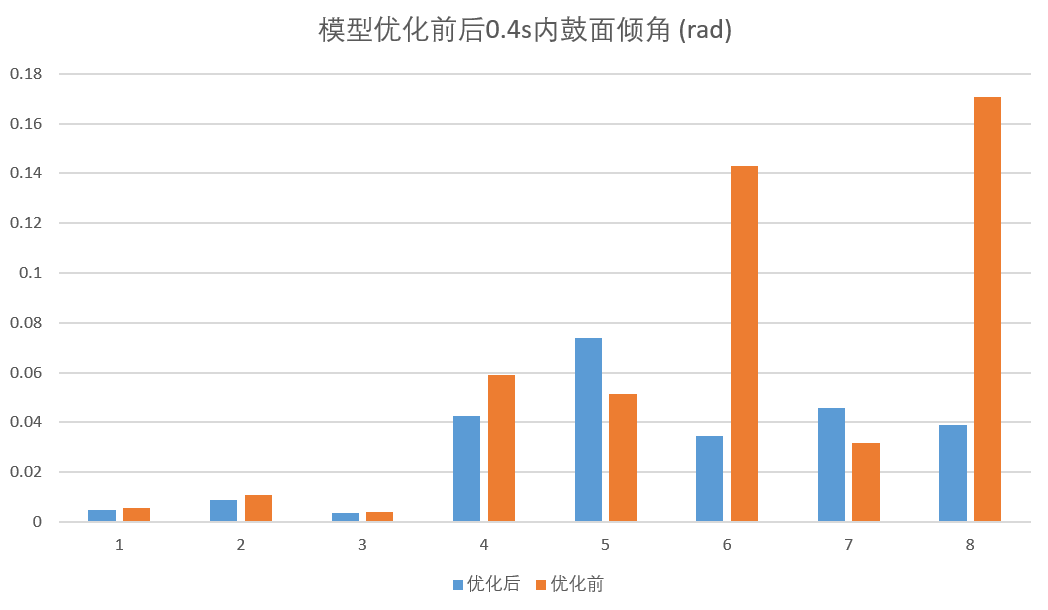
\includegraphics[width=1.0\linewidth]{figures/6.png}
    \caption{5.3.2 实验对比图}
    \label{5.3.2 实验对比图}
\end{figure}
%\znq{麻烦用问题2的数据再代入问题3的模型求一遍最后的偏转角}
\subsubsection{模型分析}

通过将问题2中的特殊情况代入问题3模型的验证过程。我们发现对于不同的情况,与模型优化前相比,采用我们优化后的策略,大都能够得到较好的效果。在这个运动过程中,鼓面会在一个较小的范围内运动,最终能够在要求时间内较为稳定地达到几乎水平的状态,这样只需要较小的位移便可以实现连续垫球不掉落。于此同时,这种方案可以保证最终状态的角速度较小,继而当球不精准落在鼓心时,可以减少对于球的运动所造成的影响。我们的模型还考虑了心理学与神经科学的研究结果,可操作性较强。

在实验中我们惊喜地发现,我们策略产生的结果对于初始状态与结束时间不敏感,对于作用力的大小也不敏感,这是一个十分优良的性质。有了这条性质,便可以在一定程度上弥补人的反应时间的影响,并且可以适应更多不同的情况。

\subsection{问题4:特殊情况:给定条件下的鼓面调整}
\subsubsection{建立模型}
这一问的特殊情况,其特征有两个,第一为转动较小的角度的控制,第二为球飞行方向为两个队员位置的角三分线。直观图如图\ref{5.4.1 角三分线示意图}所示。
\begin{figure}[h!]
    \centering
    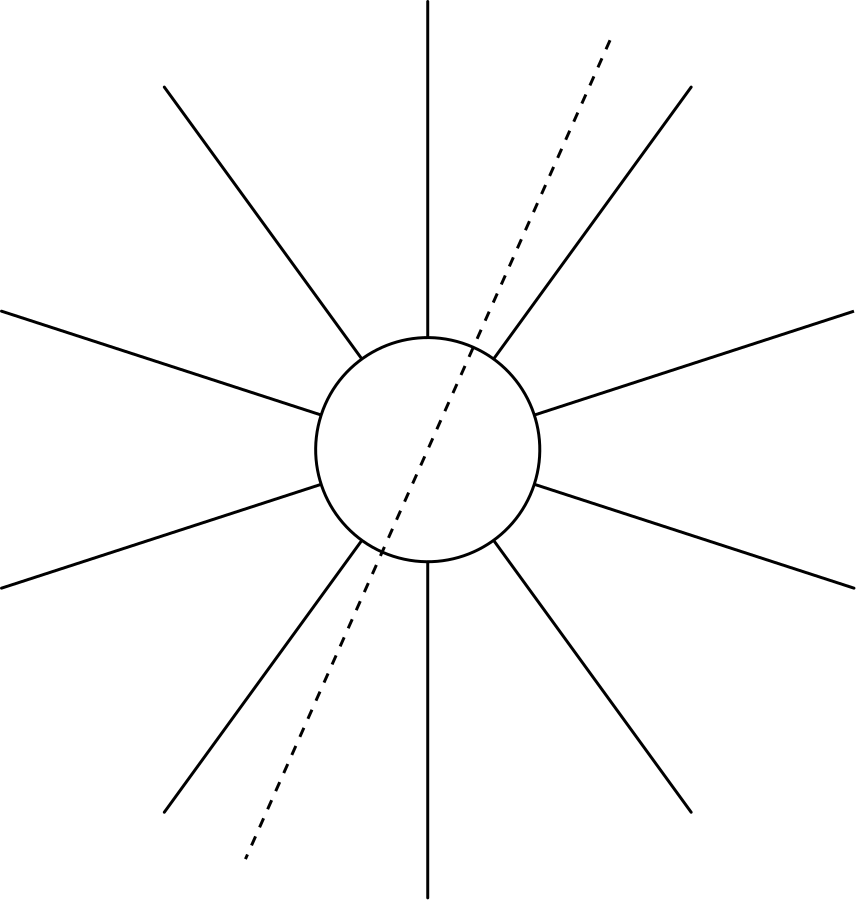
\includegraphics[width=0.4\linewidth]{figures/4.png}
    \caption{5.4.1 角三分线示意图}
    \label{5.4.1 角三分线示意图}
\end{figure}

角三分线意味着为了使得球竖直上弹,鼓转动的方向必须与球飞行的方向相同,即转轴垂直于两个队员的角三分线。这也就要求着所有队员的合力矩应该垂直于球飞行的方向。转动较小的角度意味着可以忽略拉力的水平分量对于合力矩的作用,我们也近似的忽略了鼓运动过程中由于位置变化和鼓面转动对于鼓受力方向产生的影响。在只考虑拉力竖直分量对力矩的影响的模型下,每一个受力点相对于质心的力矩均垂直于受力点到质心的连线。

我们仍然沿用类似问题1的模型。根据问题1的结论,在碰撞之后,鼓在竖直方向上的速度几乎为0,我们在这一问中可以近似取为0。因此整个过程分为三部分,具体如下:
\begin{enumerate}
    \item 自由落体(0到$t_1$)
    
    此时鼓向下做自由落体运动,可以认为是团队成员在上一次碰撞后有短暂的间歇。
    \item 匀加速直线运动($t_1$到$t_1+t_2$)
    
    此时团队成员开始用力,鼓经历匀加速直线运动到达接近碰撞点的位置,这一阶段的加速度为$a$(以向上为正方向)。
    
    \item 调整角度($t_1+t_2$到$t_1+t_2+0.1$s)
    
    由于需要转过的角度很小,这一阶段只有两位团队成员发力,继而产生力矩对鼓面角度进行调整,随即转动0.5°。经过球与鼓心的碰撞,可以修正球与竖直方向1°偏角。
    
    如图所示,此时8位团队成员停止拉绳,只有2位团队成员继续向上拉绳,不妨设该拉力的竖直分量位$F$。显然即使鼓面转过0.5°时,此时鼓面与水平面的夹角相较于拉鼓的绳子与水平面的夹角,仍然是一个小量。又因为第三阶段中,鼓的水平速度为0,在粗略的近似下,我们可以忽略此阶段鼓水平位置的变化。由于此阶段中,用于修成角度的力的大小较小,可以将此阶段竖直方向的运动视为竖直上抛。
    
\end{enumerate}

\subsubsection{模型求解}
该过程具体受力情况如图\ref{5.4.2 具体受力情况}所示。

\begin{figure}[h!]
    \centering
    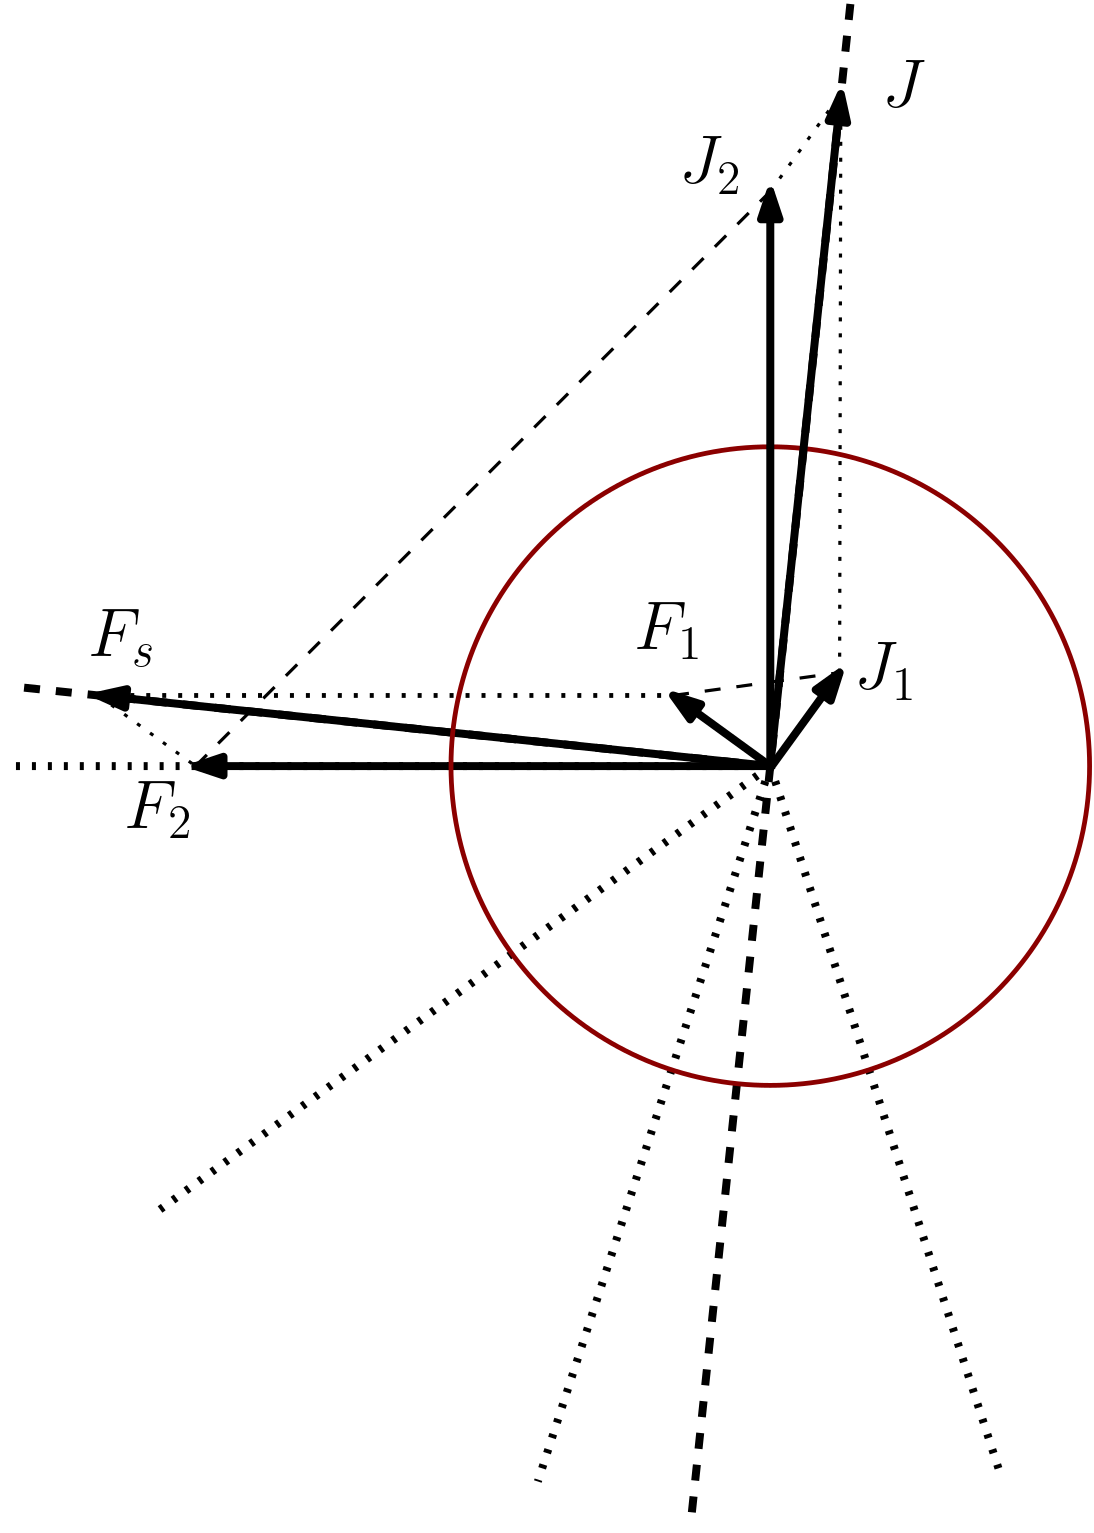
\includegraphics[width=0.4\linewidth]{figures/5.png}
    \caption{5.4.2 具体受力情况}
    \label{5.4.2 具体受力情况}
\end{figure}
\begin{enumerate}[(1)]
    \item 不妨设整个过程所用总时间为$T$,显然有
    $$T = t_1 +t_2 +0.1$$
    \item 第一阶段鼓自由落体运动,结束时速度$v_{1f}$,位置$y_{1f}$
    $$v_{1f} = -gt_1$$
    $$y_{1f} = -\frac{1}{2} g t_1^2$$
    \item 第二阶段鼓匀加速直线运动,结束时到达$y_{2f}$,速度为$v_{2f}$
    $$y_{2f} = y_{1f} + v_{1f}t_2 + \frac{1}{2}a t_2^2$$
    $$v_{2f} = v_{1f} + a t_2$$
    \item 第三阶段鼓做匀角加速旋转,设合力矩为$J$,则满足,
    $$y_{2f} + \frac{v_{2f}^2}{2g} = 0$$
    $$I\beta = J$$
    $$\Delta \Theta = \frac{1}{2}\beta \times 0.1^2$$
   
   \item
   上式中$\Delta \Theta$表示鼓面相对水平面转过的角度,在此处取0.5°。
我们发现上述模型中未知量的数量比方程数量多1个,因此我们可以添加限制条件,我们为$v_{2f}$赋予若干有意义的合理的值进行数值计算。我们使用MATLAB对于不同$v_{2f}$的情况进行方程求解,具体代码如附录中问题4代码所示。

经实验,我们发现当$v_{2f}=0.8$m/s时,各个物理量的解均合理,于是我们采用表\ref{table:result3}这组解,即:


\begin{table} [!h]
\begin{center}
\vspace{-0.1in}
\caption{问题4计算结果}
\label{table:result3}
\begin{tabular}{|c|l|l|l|l|l|l|}
\hline
$t_1$ & $t_2$ & $a_0$ & $v_{1f}$ & $v_{2f}$ & $y_{1f}$ & $y_{2f}$\\
\hline
 0.0816   & 0.5182 &   3.0875&   -0.8000    &0.8000&   -0.0327  & -0.0327\\
\hline
\end{tabular}
\vspace{-0.2in}
\end{center}
\end{table}

\item
考虑求解调整角度的过程,联立上式可得,
$$\beta = 1.7453 s^{-2}$$
$$J = I\beta = 0.1510 N\cdot m$$
\item
根据图\ref{5.4.2 具体受力情况}上的几何性质可得,
$$J_1 = 0.0257 N\cdot m$$
$$J_2 = 0.1286 N\cdot m$$
\item
考虑这两位团队成员用力的竖直方向分量,满足
$$F_i r = J_i$$
则
$$F_{1z} = 0.1285 N$$
$$F_{2z} = 0.6430 N$$
\item
不妨认为此时绳子与水平面的夹角为$\alpha$,则两位团队成员的用力大小为
$$F_{1} = F_{1z}/\alpha$$
$$F_{2} = F_{2z}/\alpha$$
\item
以$\alpha = 0.11/1.7$为例,则
$$F_{1} = 1.98 N$$
$$F_{2} = 9.94 N$$

\end{enumerate}
\subsubsection{模型分析}
上述的模型较为准确的描述了为向上抛球进行修正的过程。以$\alpha = 0.11/1.7$为例,所得到的拉力向上的分量很小,也印证了可以近似视为竖直上抛运动的假设的合理性。

当恢复系数$e$较大的时候,上述的变量组合也可以保证球下一次弹起仍然高于40cm的要求。即使遇到较小的恢复系数$e$,也可以控制末态速度,对此模型进行简单的修改。这意味着此模型有着较强的普适性。

此模型对于鼓质心运动的方法,对于人的协同性与力大小的准确性敏感性较低,这意味着即使是真实情况,也可以成功的把球弹到符合要求的高度。

但是本模型关于使鼓旋转继而微调鼓的位置的部分,对于发力时机与发力大小的同步性与准确性有着较高的要求,这意味着在实际情况中,难以利用此模型对于1°左右的偏差进行回复调整。事实上,1°左右的偏差对于球的运动影响极小,同时鼓面0.5°的旋转是人眼难以辨别的\cite{eyes},故难以控制。这意味着,问题4所述要求在实际情况下难以实现,也并不重要。

\section{模型的优缺点}
%\znq{这里我只写了一点点的梗概的内容,还需要补充和扩充}
\subsection{模型的优点}
\subsubsection{针对问题1的模型1}
\begin{enumerate}[(1)]
    \item 
球和鼓的运动都只涉及匀加速运动与自由落体运动,计算简单。
\item
球和鼓的运动周期最短,团队成员发力的大小最小,消耗能量最少。
\item
鼓在垂直方向上的移动的距离较短,对绳的牵拉程度较小,团队成员在拉绳时不易失控。
%\znq{加油}
%\lhp{stable}
\end{enumerate}
\subsubsection{针对问题2的模型2}
\begin{enumerate}[(1)]
    \item 
对于对称性的问题,鼓面倾斜角度计算时不依赖于小角近似,可对于任意角度求解。
\item
我们的模型与算法对于对称的情况有较强的可拓展性,可以利用相同的算法实现物理引擎。
%物理引擎是啥 没文化的人流下泪水
%\znq{物理引擎可以用在3D建模中,比如用在游戏中,或者是用在人造卫星的电脑模拟啊}
%\lhp{啊 a}
\item 对于非对称性的问题,不需要分析复杂的刚体定点转动问题,巧妙的利用了角度微元为矢量的特性,得到了精确度足够高的结果。
\end{enumerate}
\subsubsection{针对问题3的模型1和模型2的组合}
\begin{enumerate}[(1)]
\item
我们的模型抓住了主要特征,对于结果影响不大但是比较复杂的部分,进行有效的近似,将问题简单化。
\item
我们的模型对于团队成员具体力的大小不敏感,保证即使发力失误也可保证鼓面较为平稳的运动。
\item
我们的模型对于团队成员的初始状态不敏感。在人类神经学的基础上,团队成员只要对自己的行动进行合适调整,就可以保证鼓面较为平稳的运动。

\item
以上两个不敏感的特性使得其可以保证鼓可以平稳运动,进而保证项目的稳定进行。

\end{enumerate}
\subsubsection{针对问题4的模型模型3}
\begin{enumerate}[(1)]
\item
我们的模型将运动过程简化,分为3个阶段,易于计算和分析。
\item
我们的模型对于每一位团队成员的行动做了明确的安排,易于实践。

\end{enumerate}
\subsection{模型的缺点}
\subsubsection{针对问题1的模型1}
\begin{enumerate}[(1)]
    \item 
实际情况下,团队成员难以实现对于发力时间、发力大小的精准控制,因此难以保证鼓的匀加速直线运动。
\item
为了使得能量消耗最低,此运动中一周期内的某段持续时间过短,低于人的正常反应时间,使得实际操作中难以实现。

\end{enumerate}
\subsubsection{针对问题2的模型2}
\begin{enumerate}[(1)]
    \item 
对于我们所定义的不对称的情况,我们的算法只支持小角度情况下的运算,可拓展性较差。

\end{enumerate}
\subsubsection{针对问题3的模型1和模型2的组合}
\begin{enumerate}[(1)]
    \item 
实际操作中,鼓的旋转速度较快,团队成员可能较难控制。
\item 
实际操作中,不同团队成员的反应时间可能存在一定偏差。
\item
但是在实际操作中,以上两缺点通过团队成员的联系与配合,都可以消除。
\end{enumerate}
\subsubsection{针对问题4的模型模型3}
\begin{enumerate}[(1)]
    \item 
    我们的方案对团队成员动作的步性与准确性有着较高的要求,这意味着在实际情况中,难以利用此模型对小角度的偏差进行调整。
\end{enumerate}
\section{结论}

本文基于同心鼓游戏中颠球次数尽可能多的目标,对该项目中球与鼓的受力与运动进行研究,综合考虑人的反应能力、控制能力等综合生理要素,建立符合该项目进行过程的物理模型,研究团队成员的最佳行动方案。对于题目中的四个问题,本文在合理假设的基础上,依次给出了完备的、可实施的解决方案。

本文建立合适的物理模型,对鼓和球进行运动受力分析,兼考虑到团队成员发力的时间、大小的误差,针对不同情况下的误差,对团队成员的行动进行调整。我们的方案总体上有较好的优化效果,且可投入实践。

而实际上,该项目在实际中会有更多的影响因素,如风力、空气阻力,以及不同团队成员的身高差异。本文的工作在这些方面还具有一定的研究、拓展空间。



%\znq{9.15 1:25, I am dying, plz help me!}



\clearpage
\bibliographystyle{plain}
\bibliography{reference}
\newpage
\appendix
\section*{附录}
\begin{appendix}
\section{问题1代码}
\lstset{breaklines}
\begin{lstlisting}[language=Matlab,numbers=left, numberstyle=\tiny,keywordstyle=\color{blue!70},commentstyle=\color{red!50!green!50!blue!50},frame=shadowbox, rulesepcolor=\color{red!20!green!20!blue!20}] 
syms t1 t2 v0 v1 v2 a;
e = 0.7;
m = 0.27;
M = 3.6;
h = 0.4;
g = 9.8;
e1 = e*(v0 + v2 + a*t2) + v1 - v0;
e2 = 2*m*v0 + M*v1 - M*(v2 + a*t2);
e3 = 2*v0/g - t1 -t2;
e4 = (v0-v1)*t1 + (v0-v1)^2/(2*(g+a)) - h;
e5 = v1*(t1+t2) + (1/2) * a * t2^2 - 0.5 * g * t1^2 -g*t1*t2;
e6 = v1 - g*t1 -v2;
[t10, t20, v00, v10, v20, a0] = solve(e1,e2,e3,e4,e5,e6,t1,t2,v0,v1,v2,a);
T0 = eval(t10(1,1) + t20(1,1))
double([t10, t20, v00, v10, v20, a0])
yd1f = v10(1,1)*t10 - 0.5*g*t10(1,1)*t10(1,1);
double(yd1f)
% 第一组为有意义的解
% v0为球弹起来的速度 v1为碰后鼓的速度 v2为鼓上抛结束后的速度
% 正方向向上
\end{lstlisting}

\section{问题2与问题3的实验数据}
\lstset{breaklines}
\begin{lstlisting}[language=Matlab,numbers=left, numberstyle=\tiny,keywordstyle=\color{blue!70},commentstyle=\color{red!50!green!50!blue!50},frame=shadowbox, rulesepcolor=\color{red!20!green!20!blue!20}] 
1
F = [90,80,80,80,80,80,80,80];
activate = [0,0,0,0,0,0,0,0];
bias = pi/4;

2
F = [90,90,80,80,80,80,80,80];
activate = [0,0,0,0,0,0,0,0];
bias = pi/8;

3
F = [90,80,80,90,80,80,80,80];
activate = [0,0,0,0,0,0,0,0];
bias = -pi/8;

4
F = [80,80,80,80,80,80,80,80];
activate = [1,0,0,0,0,0,0,0];
bias = pi/4;

5
F = [80,80,80,80,80,80,80,80];
activate = [1,1,0,0,0,0,0,0];
bias = pi/8;

6
F = [80,80,80,80,80,80,80,80];
activate = [1,0,0,1,0,0,0,0];
bias = -pi/8;

7
F = [90,80,80,80,80,80,80,80];
activate = [1,0,0,0,0,0,0,0];
bias = pi/4;

8
F = [90,80,80,90,80,80,80,80];
activate = [0,1,0,0,1,0,0,0];
bias = ;

9
F = [90,80,80,90,80,80,80,80];
activate = [0,0,0,0,1,0,0,1];
bias = -pi/8;

\end{lstlisting}

\section{问题2代码}
\lstset{breaklines}
\begin{lstlisting}[language=Matlab,numbers=left, numberstyle=\tiny,keywordstyle=\color{blue!70},commentstyle=\color{red!50!green!50!blue!50},frame=shadowbox, rulesepcolor=\color{red!20!green!20!blue!20}] 
 % 以对称轴为y轴,则各个力位于(4i/pi + bias)的位置
F = [80,80,80,80,80,80,80,80];
activate = [1,1,0,0,0,0,0,0];
bias = pi/8;
theta = [];
I = 0.0865;
for i = 1:8
    theta(1,i) = pi*i/4 +bias;
end
alpha = 0.11/1.7;
delta = 0;
omega = 0;
% first period
for i = 1:10000
    M = [0,0,0];
    for j = 1:8
        r = [0.2*sin(theta(1,j))*cos(delta), 0.2*cos(theta(1,j)),-0.2*sin(theta(1,j))*sin(delta)];
        Fj = [F(1,j)*sin(theta(1,j))*cos(alpha), F(1,j)*cos(theta(1,j))*cos(alpha), F(1,j)*sin(alpha)];
        if activate(1,j)==1
            M = M + cross(r,Fj);   
        end
    end
    delta = delta + omega* 0.1/10000;
    omega = omega + M(1,2)/I * 0.1/10000;
end
%second period
for i = 1:(10000)
    M = [0,0,0];
    for j = 1:8
        r = [0.2*sin(theta(1,j))*cos(delta), 0.2*cos(theta(1,j)),-0.2*sin(theta(1,j))*sin(delta)];
        Fj = [F(1,j)*sin(theta(1,j))*cos(alpha), F(1,j)*cos(theta(1,j))*cos(alpha), F(1,j)*sin(alpha)];
        % r
        % Fj
        M = M + cross(r,Fj); 
    end
    delta = delta + omega* 0.1/10000;
    omega = omega + M(1,2)/I * 0.1/10000;
end
omega
delta
\end{lstlisting}








\section{问题3代码}
\lstset{breaklines}
\begin{lstlisting}[language=Matlab,numbers=left, numberstyle=\tiny,keywordstyle=\color{blue!70},commentstyle=\color{red!50!green!50!blue!50},frame=shadowbox, rulesepcolor=\color{red!20!green!20!blue!20}] 
% 主要思想是,在鼓上升的过程中,减小鼓的倾斜角
% 以对称轴为y轴,则各个力位于(4i/pi + bias)的位置
F = [80,80,80,80,80,80,80,80];
activate = [1,1,0,0,0,0,0,0];
bias = pi/8;
theta = [];
I = 0.0865;
for i = 1:8
    theta(1,i) = pi*i/4 +bias;
end
alpha = 0.14/1.7;
delta = 0;
omega = 0;

% period 1
for i = 1:10000
    M = [0,0,0];
    for j = 1:8
        r = [0.2*sin(theta(1,j))*cos(delta), 0.2*cos(theta(1,j)),-0.2*sin(theta(1,j))*sin(delta)];
        Fj = [F(1,j)*sin(theta(1,j))*cos(alpha), F(1,j)*cos(theta(1,j))*cos(alpha), F(1,j)*sin(alpha)];
        if activate(1,j)==1
            M = M + cross(r,Fj);   
        end
    end
    delta = delta + omega* 0.1/10000;
    omega = omega + M(1,2)/I * 0.1/10000;
end
"period 1"
["omega","delta";omega,delta]
% period 2
for i = 1:(10000)
    M = [0,0,0];
    for j = 1:8
        r = [0.2*sin(theta(1,j))*cos(delta), 0.2*cos(theta(1,j)),-0.2*sin(theta(1,j))*sin(delta)];
        Fj = [F(1,j)*sin(theta(1,j))*cos(alpha), F(1,j)*cos(theta(1,j))*cos(alpha), F(1,j)*sin(alpha)];
        M = M + cross(r,Fj); 
    end
    delta = delta + omega* 0.1/10000;
    omega = omega + M(1,2)/I * 0.1/10000;
end
"period 2"
["omega","delta";omega,delta]

% he noticed he was early and dimished his force
F_backup = F;
for i = 1:8
    if activate(1,i) ==1
        F(1,i) = 1.5*F(1,i);
    end
end
% period 3
for i = 1:(30000)
    M = [0,0,0];
    for j = 1:8
        r = [0.2*sin(theta(1,j))*cos(delta), 0.2*cos(theta(1,j)),-0.2*sin(theta(1,j))*sin(delta)];
        Fj = [F(1,j)*sin(theta(1,j))*cos(alpha), F(1,j)*cos(theta(1,j))*cos(alpha), F(1,j)*sin(alpha)];
        M = M + cross(r,Fj); 
    end
    delta = delta + omega* 0.1/10000;
    omega = omega + M(1,2)/I * 0.1/10000;
end
"period 3"
["omega","delta";omega,delta]
\end{lstlisting}


\section{问题4代码}
\lstset{breaklines}
\begin{lstlisting}[language=Matlab,numbers=left, numberstyle=\tiny,keywordstyle=\color{blue!70},commentstyle=\color{red!50!green!50!blue!50},frame=shadowbox, rulesepcolor=\color{red!20!green!20!blue!20}] 
theta = 0.5/180 * pi;
g = 9.8;
h = 0.6;
I = 0.0865;
T = 2*sqrt(2*h/g);
syms t1 t2 a v1f y1f y2f v2f;
e1 = t1+t2+0.1-T;
e2 = v1f+g*t1;
e3 = y1f+0.5*g*t1^2;
e4 = y1f +v1f *t2+0.5*a*t2^2-y2f;
e5 = v2f-v1f-a*t2;
e6 = y2f + v2f^2/2/g;
e7 = v2f -0.8;
[t10, t20, a0, v1f0, v2f0, y1f0, y2f0] = solve(e1,e2,e3,e4,e5,e6,e7,t1, t2, a, v1f, v2f, y1f, y2f);
eval([t10, t20, a0, v1f0, v2f0, y1f0, y2f0])
\end{lstlisting}


\end{appendix}

\end{document}
